\subsection{Transistor steuert LED} % (fold)
\label{sub:Transistor_steuert_LED}
\begin{frame}
    \frametitle{Transistor steuert LED}
    \framesubtitle{Schaltplan}
    \begin{figure}[H]
    \begin{center}
            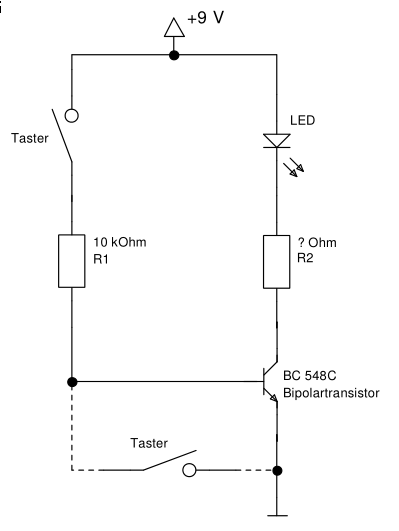
\includegraphics[scale=0.35]{./img/schaltungen/transistorLED_1.png}
    \end{center}
    \end{figure}
\end{frame}
\begin{frame}
    \frametitle{Transistor steuert LED}
    \begin{columns}[c]
    \column{.5\textwidth}
        \begin{figure}[H]
        \begin{center}
                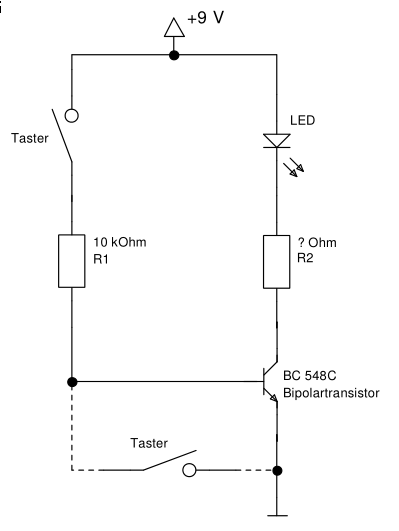
\includegraphics[scale=0.35]{./img/schaltungen/transistorLED_1.png}
        \end{center}
        \end{figure}
    \column{.6\textwidth}
    \begin{alertblock}{Achtung!}
         \begin{itemize}
             \item Zu hohe Spannung kann LED beschädigen
         \end{itemize}
    \end{alertblock}
    \pause
    \begin{block}{Widerstand $R2$}
         \begin{itemize}
             \item Aus Spezifikationen für die blaue LED:
                \begin{align*}
                    U_{max} &= 4.1V \\
                    I_{max} &= 20mA \\
                    \rightarrow R_{R2} &\geq \frac{9V - 4.1V}{20mA}\geq245\Omega
                \end{align*}
             \item Verwendet wurde $475 \Omega$ Widerstand
         \end{itemize}
    \end{block}
    \end{columns}
\end{frame}

\begin{frame}
    \frametitle{Transistor steuert LED}
    \begin{columns}[c]
    \column{.5\textwidth}
        \begin{figure}[H]
        \begin{center}
                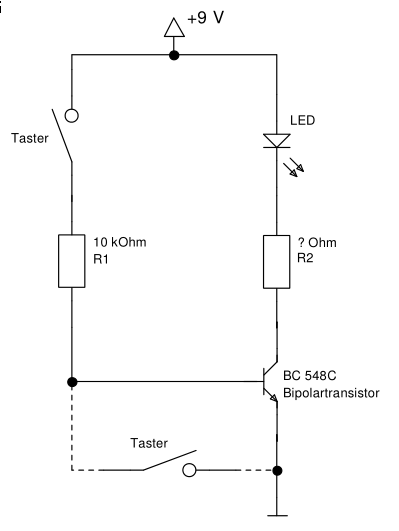
\includegraphics[scale=0.35]{./img/schaltungen/transistorLED_1.png}
        \end{center}
        \end{figure}
    \column{.6\textwidth}
    \begin{block}{Funktionsweise}
         \begin{itemize}
            \item Schalter offen:
            \begin{itemize}
                \item kein Strom an Basis
                \item kein Durchlass
                \item kein Strom, LED leuchtet nicht
            \end{itemize}
            \pause
            \item Schalter gedrückt:
            \begin{itemize}
                \item Strom and Basis
                \item Strom von Quelle zur Masse
                \item LED leuchtet
            \end{itemize}
         \end{itemize}
    \end{block}
    \end{columns}
\end{frame}

\begin{frame}
    \frametitle{Transistor steuert LED}
    \begin{columns}[c]
    \column{.5\textwidth}
        \begin{figure}[H]
        \begin{center}
                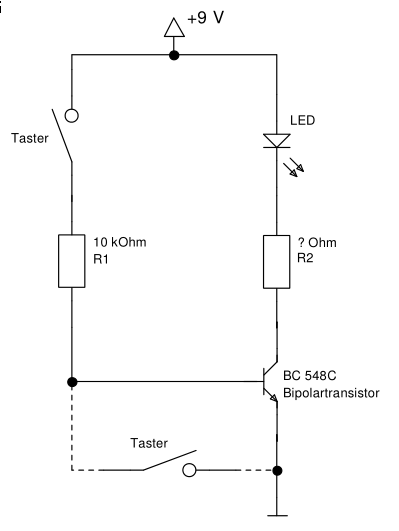
\includegraphics[scale=0.35]{./img/schaltungen/transistorLED_2.png}
        \end{center}
        \end{figure}
    \column{.6\textwidth}
    \begin{block}{Umbau}
        \begin{itemize}
            \item Schalter wurde zwischen Basis und Emitter gebaut
        \end{itemize}    
    \end{block}
    \begin{block}{Funktionsweise}
        \begin{itemize}
            \item Schalter offen:
            \begin{itemize}
                \item Strom an Basis
                \item LED leuchtet
            \end{itemize}
            \pause
            \item Schalter gedrückt:
            \begin{itemize}
                \item (fast) Kurzschluss zwischen Quelle und Masse
                \item geringer Spannungsabfall an Transistor $\rightarrow$ wird
                nicht geschaltet
                \item kein Strom durch LED
            \end{itemize}
        \end{itemize}
    \end{block}
    \end{columns}
\end{frame}

\begin{frame}
    \frametitle{Transistor steuert LED}
    \begin{columns}[c]
    \column{.5\textwidth}
        \begin{figure}[H]
        \begin{center}
                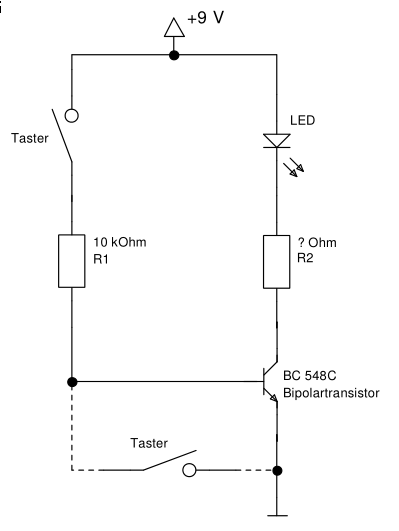
\includegraphics[scale=0.35]{./img/schaltungen/transistorLED_2.png}
        \end{center}
        \end{figure}
    \column{.6\textwidth}
    \begin{block}{Erkentnisse}
    \begin{itemize}
        \item Transistor kann einfache An- bzw Aus-Schaltung realisieren
        \item Aus-Schaltung kann nicht mit Taster alleine gebaut werden
    \end{itemize}
    \end{block}
    \end{columns}
\end{frame}
% section Transistor steuert LED (end)
